% !TEX program = xelatex
\documentclass[10pt,a4paper]{article}

\usepackage[a4paper,top=0.66in,bottom=0.61in,left=0.76in,right=0.76in,headheight=20pt,headsep=10pt,footskip=20pt]{geometry}
\usepackage{fontspec}
\usepackage{amsmath}
\setmonofont{Courier New}
\usepackage{microtype}
\usepackage{graphicx}
\graphicspath{{report/assets/}{assets/}}
\usepackage{booktabs}
\usepackage{tabularx}
\usepackage{array}
\usepackage{enumitem}
\usepackage{fancyhdr}
\usepackage{lastpage}
\usepackage{hyperref}
\usepackage[table]{xcolor}
\usepackage[most]{tcolorbox}
\usepackage{tikz}
\usepackage{ragged2e}
\usepackage{polyglossia}
\setdefaultlanguage{hebrew}
\setotherlanguage{english}
\newfontfamily\hebrewfont[Script=Hebrew]{Arial Hebrew}
\newfontfamily\hebrewfontsf[Script=Hebrew]{Arial Hebrew}
\newfontfamily\englishfont{Arial}
\newfontfamily\englishfontsf{Arial}

\definecolor{Navy}{HTML}{17233B}
\definecolor{Blue}{HTML}{2E74B5}
\definecolor{PaleBlue}{HTML}{EAF3FB}
\definecolor{Ink}{HTML}{18212F}
\definecolor{Muted}{HTML}{5E6B7C}
\definecolor{Light}{HTML}{F2F4F7}
\definecolor{Green}{HTML}{0A7D54}
\definecolor{Amber}{HTML}{A15C00}
\definecolor{Rule}{HTML}{D7DEE8}

\hypersetup{
  colorlinks=true,
  urlcolor=Blue,
  linkcolor=Blue,
  unicode=true,
  pdftitle={Airfoil Explorer - DRL x LBM Design Space},
  pdfauthor={Eden Menachem Golan, 211587894},
  pdfsubject={AI course final-project report - Hebrew submission}
}

\pagestyle{empty}

\setlength{\parindent}{0pt}
\setlength{\parskip}{3.8pt}
\setlength{\tabcolsep}{5pt}
\renewcommand{\arraystretch}{1.15}
\setlist[itemize]{rightmargin=1.25em,leftmargin=0pt,itemsep=1.7pt,topsep=2pt,parsep=0pt}
\setlist[itemize,1]{label=\textcolor{Blue}{\small\ensuremath{\bullet}}}

\newcommand{\eyebrow}[1]{\textcolor{Blue}{\fontsize{7.5}{8}\selectfont\bfseries #1}\par\vspace{2pt}}
\newcommand{\pagetitle}[3]{%
  \eyebrow{\textenglish{#1 / 04}}%
  {\color{Blue}\fontsize{16}{18}\selectfont\bfseries #2\par}%
  \vspace{2pt}\textcolor{Rule}{\rule{\textwidth}{0.7pt}}\vspace{2pt}\par
  {\color{Muted}\fontsize{9}{11}\selectfont #3\par}\vspace{4pt}%
}
\newcommand{\sectiontitle}[1]{\vspace{3pt}{\color{Navy}\fontsize{11.2}{13}\selectfont\bfseries #1\par}\vspace{1pt}}
\newcommand{\smallbody}{\fontsize{8.55}{10.35}\selectfont}
\newcommand{\tinybody}{\fontsize{7.45}{9}\selectfont}
\newcommand{\statuspassed}{\textcolor{Green}{\bfseries עבר}}

\newtcolorbox{callout}[1][]{
  enhanced,
  colback=PaleBlue,
  colframe=Rule,
  boxrule=0.45pt,
  arc=3mm,
  left=3mm,right=3mm,top=2.2mm,bottom=2.2mm,
  before skip=3pt,after skip=4pt,
  #1
}
\newtcolorbox{softcard}[1][]{
  enhanced,
  colback=Light,
  colframe=Rule,
  boxrule=0.4pt,
  arc=2.5mm,
  left=2.4mm,right=2.4mm,top=2mm,bottom=2mm,
  #1
}

\newcolumntype{Y}{>{\RaggedLeft\arraybackslash}X}
\newcolumntype{L}[1]{>{\RaggedLeft\arraybackslash}p{#1}}
\newcolumntype{C}[1]{>{\Centering\arraybackslash}p{#1}}

\begin{document}

% PAGE 1 -- introduction
\eyebrow{מטלת סיום - שימושים ופיתוח בעזרת בינה מלאכותית בהובלת מומחה}
{\color{Navy}\fontsize{29}{31}\selectfont\bfseries סייר פרופילי כנף\par}
{\color{Muted}\fontsize{13}{15}\selectfont מרחב תכן \textenglish{DRL x LBM}\par}
\vspace{3pt}\textcolor{Blue}{\rule{\textwidth}{1.25pt}}\vspace{4pt}

\begin{softcard}
\begin{tabularx}{\linewidth}{@{}Y Y@{}}
\eyebrow{מגיש} עדן מנחם גולן & \eyebrow{תעודת זהות} \textenglish{211587894} \\
\eyebrow{תאריך} 11 באוגוסט 2026 & \eyebrow{תוצר} אתר אינטראקטיבי פעיל
\end{tabularx}
\end{softcard}

\sectiontitle{1. מבוא למקצוע}
{\smallbody
תחום המחקר שלי הוא אווירודינמיקה חישובית ואופטימיזציה של פרופילי כנף. במהלך התזה אני משתמש בחישובי \textenglish{Computational Fluid Dynamics (CFD)} בשיטת \textenglish{Lattice Boltzmann Method (LBM)} כדי לחשב את מקדמי העילוי והגרר של פרופילי כנף. במקביל, אלגוריתם \textenglish{Deep Reinforcement Learning (DRL)} משנה את פרמטרי \textenglish{BP3333} ומחפש גאומטריות בעלות ביצועים אווירודינמיים טובים יותר. הבנת הפרויקט דורשת היכרות עם מקדמי העילוי והגרר, \textenglish{$C_l$} ו-\textenglish{$C_d$}, עם יחס היעילות \textenglish{$C_l/C_d$}, ועם השפעת תנאי הסימולציה על יכולת ההשוואה בין תוצאות.
}

\sectiontitle{הבעיה וההישג הנדרש}
{\smallbody
במהלך העבודה מחושבים עילוי וגרר עבור אלפי פרופילי כנף. המידע נשמר בריצות ניסוי נפרדות, אך אינו מוצג במאגר מאוחד, מקוטלג ונגיש. לכן קשה לזהות מגמות, להשוות בין כנפיים ולהבין כיצד שינוי בכל אחד מפרמטרי הגאומטריה משפיע על העילוי, הגרר והיעילות. בנוסף, אסור להשוות ישירות בין תוצאות שהתקבלו בתנאים פיזיקליים או נומריים שונים.
}

\begin{callout}
{\color{Navy}\bfseries\small ההישג שהוגדר}\par\vspace{1pt}
{\smallbody בניית מאגר מידע מאוחד ומקוטלג של כל פרופילי הכנף התקינים שעבורם הושלמה סימולציה. המאגר מופרד לקבוצות לפי תנאי הסימולציה, ובהם מספר ריינולדס, זווית התקפה, גודל הרשת, זמן הריצה ביחידות \textenglish{TU}, מהירות הזרימה בכניסה ותנאים פיזיקליים ונומריים נוספים. המאגר מוצג באתר אינטראקטיבי: לכל פרמטר כנף קיים מחוון, וגרירתו מציגה מיד את הכנף המחושבת הקרובה ביותר במרחב הפרמטרים ואת ערכי \textenglish{$C_l$, $C_d$, $C_l/C_d$} שלה. האתר מתעדכן אוטומטית פעם בשעה מתוצאות חדשות המועלות ל-\textenglish{W\&B}.}
\end{callout}

\sectiontitle{מדדי הצלחה והגבלות הנדסיות}
{\smallbody
\begin{itemize}
  \item כל כנף והמקדמים המוצגים לצידה מגיעים מאותה איטרציה, עם תווית ריצה ושלב.
  \item ריצות מאוחדות רק כאשר תנאי הסימולציה שלהן תואמים; תנאים לא ידועים נשמרים בנפרד.
  \item גאומטריות לא תקינות ותוצאות עונש בעלות עילוי שלילי אינן מוצגות ככנפיים תקפות.
  \item הממשק מציג תוצאות מדודות בלבד ואינו מבצע אינטרפולציה או חיזוי אווירודינמי.
  \item כשל בייצוא או באימות אינו מחליף את הגרסה הציבורית האחרונה שעברה את כל הבדיקות.
\end{itemize}
}

\newpage

% PAGE 2 -- final product
\pagetitle{02}{2. התוצר הסופי}{אתר ציבורי שמאחד את תוצאות הסימולציה ומאפשר לחקור אותן באופן אינטראקטיבי.}

\begin{center}
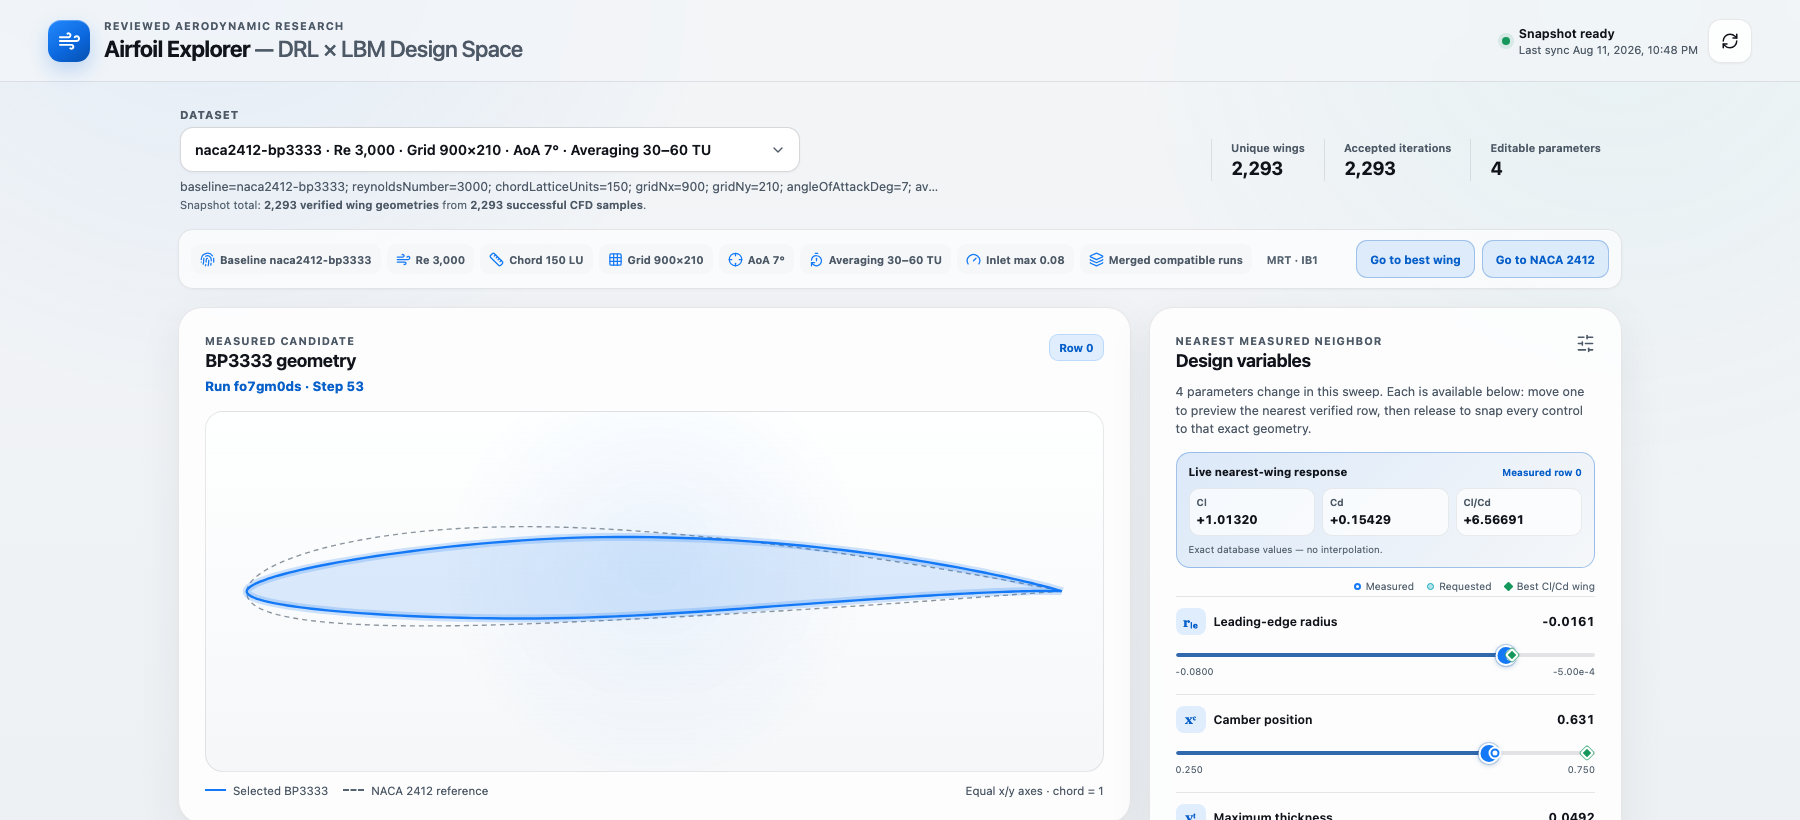
\includegraphics[width=\textwidth]{dashboard-live.png}
\vspace{-3pt}

{\color{Muted}\fontsize{7.3}{8.5}\selectfont איור 1. האתר הפעיל מציג כנף מחושבת, פרמטרים, מקדמים ותנאי סימולציה מאותה רשומת מקור.}
\end{center}
\vspace{2pt}

\begin{tabularx}{\textwidth}{@{}YYYY@{}}
\begin{softcard}\centering{\color{Blue}\fontsize{16}{17}\bfseries \textenglish{2,293}}\par{\tinybody גאומטריות כנף מאומתות}\end{softcard} &
\begin{softcard}\centering{\color{Green}\fontsize{16}{17}\bfseries \textenglish{2,293}}\par{\tinybody דגימות \textenglish{CFD} מוצלחות}\end{softcard} &
\begin{softcard}\centering{\color{Navy}\fontsize{16}{17}\bfseries \textenglish{5}}\par{\tinybody ריצות מקור שנבדקו}\end{softcard} &
\begin{softcard}\centering{\color{Amber}\fontsize{16}{17}\bfseries \textenglish{1}}\par{\tinybody קבוצת תנאים תואמת}\end{softcard}
\end{tabularx}

\sectiontitle{מהו התוצר וכיצד משתמשים בו}
{\smallbody
האתר הוא ממשק חקירה למאגר הכנפיים. בראש העמוד בוחרים קבוצת נתונים; כל קבוצה מכילה רק ריצות בעלות תנאים פיזיקליים ונומריים תואמים. לאחר הבחירה מוצגים פרופיל הכנף, ערכי \textenglish{$C_l$}, \textenglish{$C_d$} ו-\textenglish{$C_l/C_d$}, תנאי הסימולציה, ומזהי הריצה והשלב ב-\textenglish{W\&B}. בצד הכנף מופיעים רק הפרמטרים שהשתנו באותה קבוצת ניסויים.
}

{\smallbody
\begin{itemize}
  \item \textbf{גרירה:} הזזת מחוון משנה את נקודת הבקשה ומחפשת בזמן אמת את הכנף המחושבת הקרובה ביותר. הכנף וכל שלושת המדדים מתעדכנים יחד.
  \item \textbf{שחרור:} כל המחוונים נצמדים לערכים המדויקים של אותה כנף. כך ברור שהערכים המוצגים נמדדו בסימולציה ולא חושבו באינטרפולציה.
  \item \textbf{ניווט:} כפתורים ייעודיים עוברים לכנף בעלת יחס \textenglish{$C_l/C_d$} הגבוה ביותר או לפרופיל הייחוס \textenglish{NACA2412}. סמנים ירוקים מציגים את מיקום הכנף היעילה על כל מחוון.
  \item \textbf{רענון:} כפתור הרענון טוען את תמונת הנתונים הציבורית החדשה ביותר; הוא אינו חושף מפתח גישה ואינו פונה ישירות ל-\textenglish{W\&B}.
\end{itemize}
}

\sectiontitle{כיצד הנתונים מגיעים לאתר}
{\smallbody
תהליך אוטומטי של \textenglish{GitHub Actions} רץ פעם בשעה וגם בהפעלה ידנית. הוא קורא מ-\textenglish{W\&B} רק את שדות ההיסטוריה הדרושים לכל איטרציה, משחזר את וקטור \textenglish{BP3333}, מסנן רשומות לא תקינות, מקבץ ריצות לפי תנאי הסימולציה ומסיר כפילויות גאומטריות באופן דטרמיניסטי. לאחר מכן נוצרים קובצי \textenglish{JSON} חתומים ב-\textenglish{SHA-256}, האתר נבנה ונפרס ב-\textenglish{GitHub Pages}. אם שלב כלשהו נכשל, הפריסה המאומתת הקודמת נשארת פעילה.
}

\begin{callout}[colback=white]
{\smallbody\textbf{קישור לתוצר:} \href{https://edengol10.github.io/AI-final-course/}{\textenglish{edengol10.github.io/AI-final-course/}}. בעת הפקת הדוח המאגר הציבורי כלל 2,293 כנפיים מאומתות מחמש ריצות, בקבוצת תנאים תואמת אחת. המונים נוצרים אוטומטית בתהליך הייצוא ואינם כתובים ידנית בממשק.}
\end{callout}

\newpage

% PAGE 3 -- AI evidence
\pagetitle{03}{3. שימוש בבינה מלאכותית בפרויקט}{בינה מלאכותית כמכפיל כוח, לצד הגדרה אנושית של הפיזיקה, הנתונים וקריטריוני הקבלה.}

\sectiontitle{כיצד הבינה המלאכותית סייעה}
{\smallbody
השימוש בבינה מלאכותית שימש מכפיל כוח לאורך כל בניית האתר. היא סייעה להבין מאגר קוד מחקרי גדול בלי לשנותו, לאתר את שדות \textenglish{W\&B} הרלוונטיים, לכתוב את מייצא הנתונים והבדיקות, לבנות את ממשק \textenglish{React/TypeScript}, לנסח את חיפוש הכנף הקרובה, להגדיר תהליך פריסה שעתי ל-\textenglish{GitHub Pages}, ולבצע בדיקות נגישות, פרטיות והתנהגות בדפדפן. העבודה נשארה בגישת \textenglish{co-coding}: אני הגדרתי את התנאים הפיזיקליים, אילו נתונים מותרים לפרסום, כיצד לסנן תוצאות עונש, ומהי התנהגות נכונה של המוצר; הבינה המלאכותית האיצה את המימוש, הבדיקה והתיעוד.
}

\sectiontitle{פרומפטים מרכזיים שניתנו במהלך העבודה}
{\tinybody הניסוחים הבאים נערכו לשונית בלבד, בלי לשנות את הדרישות המקוריות.}
\begin{softcard}[colback=white]
{\tinybody
\textbf{1. ארכיטקטורה ומימוש:} "בנה אתר \textenglish{React/TypeScript/Vite} במאגר הקורס בלבד. התייחס למאגר התזה כמקור לקריאה בלבד. הוסף מייצא \textenglish{Python} לנתוני \textenglish{W\&B}, חיפוש כנף קרובה, בדיקות ופריסה אוטומטית ל-\textenglish{GitHub Pages}. אין לבצע אינטרפולציה של תוצאות אווירודינמיות." \textbf{תוצר:} שלד היישום, מייצא הנתונים ותהליך הפריסה.\par\vspace{2pt}
\textbf{2. איסוף וסיווג נתונים:} "משוך את כל איטרציות הכנף מהריצות המאושרות. השאר רק גאומטריות תקינות בעלות עילוי חיובי, ואחד ריצות רק כאשר מספר ריינולדס, הרשת, זווית ההתקפה, זמן הריצה ותנאי הזרימה תואמים. שמור לכל כנף מזהה ריצה ושלב." \textbf{תוצר:} תמונת נתונים מאומתת הכוללת 2,293 כנפיים מחמש ריצות.\par\vspace{2pt}
\textbf{3. ממשק ואימות:} "הצג בזמן גרירה את הכנף המחושבת הקרובה ואת \textenglish{$C_l$, $C_d$, $C_l/C_d$}. הוסף סימון ירוק לכנף היעילה, פרופיל ייחוס \textenglish{NACA2412}, כפתורי ניווט ורענון, ובדוק את ההתנהגות במחשב ובטלפון לפני הפריסה." \textbf{תוצר:} הממשק הפעיל ובדיקות האינטראקציה והנגישות.
}
\end{softcard}

\sectiontitle{הסקילים שבהם השתמשתי}
\begin{softcard}
{\tinybody
\textenglish{\textbf{curate-aero-wandb-data}} - מגדיר אילו שדות נמשכים מ-\textenglish{W\&B}, כיצד לשחזר את וקטור \textenglish{BP3333}, אילו רשומות לפסול, כיצד לקבץ תנאים תואמים ואילו פרטי מקור מותר לפרסם.\par\vspace{1pt}
\textenglish{\textbf{verify-airfoil-explorer}} - מגדיר בדיקות קבלה לממשק: עקביות בין הכנף והמקדמים, גרירה והצמדה, רענון, נגישות, תצוגה רספונסיבית, פרטיות ותקינות הפריסה.\par\vspace{1pt}
\textenglish{\textbf{caveman}} - מצמצם ניסוחי סטטוס טכניים ושומר עובדות, מספרים ומונחים מדויקים. הוא מתאים בעיקר לתקשורת קצרה, ולא לכתיבת הדוח עצמו.
}
\end{softcard}

\sectiontitle{ניסוי מבוקר: הפעלה רגילה לעומת \textenglish{caveman}}
{\tinybody
אותה משימה נשלחה פעמיים באותו כלי: לנסח עדכון לבודק הכולל את מספר הכנפיים והריצות, התנהגות המחוונים, העדכון השעתי והגנת הפריסה. איכות נבדקה לפי חמש דרישות: ארבע עובדות נדרשות, ללא עובדה מומצאת, וניסוח קריא.
\par}
\begin{softcard}[colback=white]
{\tinybody
\textbf{ללא הסקיל:} "עדכון סטטוס לבודק: באתר מוצגות 2,293 כנפיים מאומתות מחמש ריצות תואמות; גרירת המחוון מציגה את הכנף המחושבת הקרובה ואת המקדמים ללא אינטרפולציה; הנתונים מתעדכנים אחת לשעה; במקרה של כשל בייצוא, הגרסה המאומתת הקודמת נשארת פעילה."\par
\textbf{עם הסקיל:} "עדכון לבודק: באתר 2,293 כנפיים מאומתות מחמש ריצות תואמות. גרירת המחוון מציגה את הכנף המחושבת הקרובה ואת המקדמים ללא אינטרפולציה. הנתונים מתעדכנים פעם בשעה. כשל בייצוא משאיר את הגרסה המאומתת הקודמת פעילה."
}
\end{softcard}
{\tinybody
\rowcolors{2}{white}{Light}
\begin{tabularx}{\textwidth}{@{}L{0.23\textwidth} C{0.16\textwidth} C{0.16\textwidth} Y@{}}
\rowcolor{Navy}\color{white}\bfseries מדד & \color{white}\bfseries ללא הסקיל & \color{white}\bfseries עם הסקיל & \color{white}\bfseries משמעות \\
זמן ריצה מקצה לקצה & \textenglish{6.93 s} & \textenglish{12.41 s} & טעינת הסקיל הוסיפה תקורה במשימה קצרה \\
טוקני פלט בכל הריצה & \textenglish{101} & \textenglish{302} & כולל הודעת הפעלה וקריאת קובץ הסקיל \\
אורך התשובה הנראית & 235 תווים & 210 תווים & קיצור של \textenglish{10.6\%} \\
איכות לפי המחוון & \textenglish{5/5} & \textenglish{5/5} & כל העובדות נשמרו, ללא תוספות \\
\end{tabularx}
}
\begin{callout}[colback=white]
{\tinybody\textbf{מסקנה:} \textenglish{caveman} קיצר את התשובה הסופית, אך בניסוי חד-פעמי ופשוט זמן הריצה וצריכת הטוקנים הכוללת גדלו בגלל תקורת טעינת הסקיל. זו מדידה של שתי ריצות בלבד, ולכן היא המחשה ולא מבחן ביצועים סטטיסטי.}
\end{callout}

\newpage

% PAGE 4 -- summary
\pagetitle{04}{4. סיכום}{ההישג הנדרש הושג: מאגר מאומת, אתר אינטראקטיבי ועדכון אוטומטי של תוצאות חדשות.}

\sectiontitle{האם ההישג הנדרש הושג}
{\smallbody
כן. נבנה מאגר ציבורי מאומת שמאחד תוצאות מריצות תואמות, והאתר מאפשר לעבור בין אלפי כנפיים באמצעות מחווני הפרמטרים. בזמן גרירה מוצגות הכנף המחושבת הקרובה והמדדים \textenglish{$C_l$, $C_d$, $C_l/C_d$}; בשחרור כל המחוונים נצמדים לאותה רשומת מקור. כל כנף מסומנת במזהי ריצה ושלב. תהליך שעתי מושך תוצאות חדשות מ-\textenglish{W\&B}, מאמת אותן ומפרסם תמונת נתונים חדשה רק אם כל הבדיקות עברו. בעת הפקת הדוח הוצגו 2,293 כנפיים מאומתות מחמש ריצות.
}

\sectiontitle{תקפות פיזיקלית ובקרת איכות}
{\smallbody
הצגת תוצאות פיזיקליות דרשה יותר מבדיקה שהקוד רץ. המייצא מקבל רק ריצות מאושרות שהסתיימו, פרמטרים סופיים הנמצאים בגבולות \textenglish{BP3333}, גאומטריה תקינה ומקדמים סופיים עם עילוי חיובי. ריצות מאוחדות רק כאשר פרופיל הבסיס, מספר ריינולדס, הרשת, זווית ההתקפה, חלון המיצוע, תנאי הכניסה והגדרות הפותר תואמים. בדיקות אוטומטיות משוות את משחזר הגאומטריה ב-\textenglish{Python} וב-\textenglish{TypeScript}, בודקות את חיפוש השכן הקרוב, ומוודאות שהכנף והמקדמים מגיעים תמיד מאותה שורה.
}

\sectiontitle{מה הייתי עושה אחרת בדיעבד}
{\smallbody
הייתי מגדיר כבר בתחילת העבודה את סכמת הנתונים הציבורית, את כללי התאימות בין ריצות ואת בדיקות הקבלה, ורק לאחר מכן בונה את הממשק. בנוסף, בדיעבד לא הייתי משתמש ב-\textenglish{superpowers} בפרויקט זה. עבור משימות ממוקדות הוא הוסיף שלבי תכנון, פיצול ובקרה שלא תמיד תרמו לתוצאה, והאריך את זמני הריצה ואת צריכת הטוקנים. הייתי משתמש במיומנויות התחומיות \textenglish{curate-aero-wandb-data} ו-\textenglish{verify-airfoil-explorer} רק בנקודות שבהן הידע המדעי או בדיקות הקבלה מצדיקים את התקורה, וב-\textenglish{caveman} רק לעדכוני סטטוס קצרים.
}

\sectiontitle{מסקנה ומסירה}
\begin{tabularx}{\textwidth}{@{}Y C{1.48in}@{}}
\begin{callout}
{\smallbody
הפרויקט הראה שבינה מלאכותית יכולה לקצר משמעותית את הדרך ממידע מחקרי מפוזר למוצר הנדסי נגיש, בתנאי שהחוקר שומר בידיו את הגדרת הפיזיקה, את אישור הנתונים ואת קריטריוני האימות. לתיק ההגשה מצורפים הדוח, האתר הפעיל, צילום הממשק, קוד הפרויקט ושלושת הסקילים שתועדו.
}
\end{callout}
&
\begin{minipage}[c]{1.42in}
\centering

\includegraphics[width=0.72in]{public-site-qr.png}\par
\vspace{1pt}{\tinybody\bfseries סייר פרופילי הכנף החי}\par
\href{https://edengol10.github.io/AI-final-course/}{\fontsize{6.2}{7}\selectfont\textenglish{edengol10.github.io}}\par
\href{https://edengol10.github.io/AI-final-course/}{\fontsize{6.2}{7}\selectfont\textenglish{AI-final-course}}
\end{minipage}
\end{tabularx}

\end{document}
